\documentclass[10pt]{article}\usepackage[]{graphicx}\usepackage[]{color}
% maxwidth is the original width if it is less than linewidth
% otherwise use linewidth (to make sure the graphics do not exceed the margin)
\makeatletter
\def\maxwidth{ %
  \ifdim\Gin@nat@width>\linewidth
    \linewidth
  \else
    \Gin@nat@width
  \fi
}
\makeatother

\definecolor{fgcolor}{rgb}{0.345, 0.345, 0.345}
\newcommand{\hlnum}[1]{\textcolor[rgb]{0.686,0.059,0.569}{#1}}%
\newcommand{\hlstr}[1]{\textcolor[rgb]{0.192,0.494,0.8}{#1}}%
\newcommand{\hlcom}[1]{\textcolor[rgb]{0.678,0.584,0.686}{\textit{#1}}}%
\newcommand{\hlopt}[1]{\textcolor[rgb]{0,0,0}{#1}}%
\newcommand{\hlstd}[1]{\textcolor[rgb]{0.345,0.345,0.345}{#1}}%
\newcommand{\hlkwa}[1]{\textcolor[rgb]{0.161,0.373,0.58}{\textbf{#1}}}%
\newcommand{\hlkwb}[1]{\textcolor[rgb]{0.69,0.353,0.396}{#1}}%
\newcommand{\hlkwc}[1]{\textcolor[rgb]{0.333,0.667,0.333}{#1}}%
\newcommand{\hlkwd}[1]{\textcolor[rgb]{0.737,0.353,0.396}{\textbf{#1}}}%
\let\hlipl\hlkwb

\usepackage{framed}
\makeatletter
\newenvironment{kframe}{%
 \def\at@end@of@kframe{}%
 \ifinner\ifhmode%
  \def\at@end@of@kframe{\end{minipage}}%
  \begin{minipage}{\columnwidth}%
 \fi\fi%
 \def\FrameCommand##1{\hskip\@totalleftmargin \hskip-\fboxsep
 \colorbox{shadecolor}{##1}\hskip-\fboxsep
     % There is no \\@totalrightmargin, so:
     \hskip-\linewidth \hskip-\@totalleftmargin \hskip\columnwidth}%
 \MakeFramed {\advance\hsize-\width
   \@totalleftmargin\z@ \linewidth\hsize
   \@setminipage}}%
 {\par\unskip\endMakeFramed%
 \at@end@of@kframe}
\makeatother

\definecolor{shadecolor}{rgb}{.97, .97, .97}
\definecolor{messagecolor}{rgb}{0, 0, 0}
\definecolor{warningcolor}{rgb}{1, 0, 1}
\definecolor{errorcolor}{rgb}{1, 0, 0}
\newenvironment{knitrout}{}{} % an empty environment to be redefined in TeX

\usepackage{alltt}
\usepackage{graphicx, verbatim}
\usepackage{amsmath}
\usepackage{amssymb}
\usepackage{amscd}
\usepackage{lipsum}
\usepackage{blindtext}
\usepackage{todonotes}
\usepackage[tableposition=top]{caption}
\usepackage{ifthen}
\usepackage[utf8]{inputenc}
\usepackage{graphicx}
\usepackage{caption}
\setlength{\textwidth}{6.5in} 
\setlength{\textheight}{9in}
\setlength{\oddsidemargin}{0in} 
\setlength{\evensidemargin}{0in}
\setlength{\topmargin}{-1.5cm}
\setlength{\parindent}{0cm}
\usepackage{setspace}
\usepackage{float}
\usepackage{amssymb}
\usepackage[utf8]{inputenc}
\usepackage{fancyhdr}
\usepackage{tabularx}

\usepackage{hyperref}
\hypersetup{
  colorlinks   = true, %Colours links instead of ugly boxes
  urlcolor     = blue, %Colour for external hyperlinks
  linkcolor    = blue, %Colour of internal links
  citecolor   = red %Colour of citations
}
%\usepackage[backend=bibtex ,sorting=none]{biblatex}
\usepackage[backend=biber ,sorting=none]{biblatex}
\bibliography{references}

\begin{filecontents*}{references.bib}

\end{filecontents*}

%\usepackage[backend=biber]{biblatex}
%\addbibresource{references.bib}


%\fancyhf{}
\rfoot{Group 2 \thepage}
\singlespacing
\usepackage[affil-it]{authblk} 
\usepackage{etoolbox}
\usepackage{lmodern}

% \makeatletter
% \renewcommand{\maketitle}{\bgroup\setlength{\parindent}{16pt}
% \begin{flushleft}
%   \textbf{\@title}
% 
%   \@author
% \end{flushleft}\egroup
% }

%\renewcommand\Authfont{\fontsize{14}{18.4}\selectfont}
%\makeatother

% \pagestyle{fancy}
% \rfoot{Page \thepage}
 %\thispagestyle{empty}
\IfFileExists{upquote.sty}{\usepackage{upquote}}{}
\begin{document}
\SweaveOpts{concordance=TRUE}


\title{\LARGE Plastic Pollution in Oceans  \\ Group 2 Report - CMM507}

\author{ALEXANDER RITCHIE, \textit{\href{1911218@rgu.ac.uk}{1911218@rgu.ac.uk}}; GEORGIOS ORFANAKIS, \textit{\href{1903446@rgu.ac.uk}{1903446@rgu.ac.uk}};KAREN JEWELL, \textit{\href{1415410@rgu.ac.uk}{1415410@rgu.ac.uk}};ROSHI SHRESTHA, \textit{\href{1903445@rgu.ac.uk}{1903445@rgu.ac.uk}};STUART WATT, \textit{\href{1501869@rgu.ac.uk}{1501869@rgu.ac.uk}}}
%ALEXANDER RITCHIE (1911218) ;GEORGIOS ORFANAKIS (1903446); KAREN JEWELL (1415410); ROSHI SHRESTHA (1903445); STUART WATT (1501869); 

\maketitle
% \begin{flushleft} \today \end{flushleft} 
\noindent\rule{16cm}{0.4pt}
%\underline{\hspace{3cm}
\ \\
%\thispagestyle{empty}

\section*{Objective}


\begin{itemize}
\item To understand the composition of plastic pollutants in the ocean
\item To understand the sources of plastic pollutants
\item To understand how plastic pollution gets distributed across the oceans
\end{itemize}

\section{Problem Statement}\label{statement}

% The command below is just to generate some text, edit here for your problem statement
%\blindtext[2]

\subsection{Overview}\label{over}

%\blindtext[2]

\subsection{Motivation}\label{mot}
%Edit here 
%\blindtext[2]

\subsection{Objectives }\label{obj}
%Edit here 
The main objectives of this project can be outlined as follows: 
\section{Research}\label{research}

 \cite{8489087}.




\section {Methods}\label{methods}

%Edit here 
%\blindtext[2]



\subsection{Data Collection}\label{dataset}



%Edit here 
%\blindtext[2]


\subsection{Exploration - Pre-processing}\label{explore}

%Edit here 
%\blindtext[2]

In this project iris was used, the dataset is made of 150 rows and four features. \\

Notice how we generate graphics within the sweave document. Check the following code, we will create a function that either finds $x^2$ or $x^3$ subject to parameters passed in the function
\begin{knitrout}
\definecolor{shadecolor}{rgb}{0.969, 0.969, 0.969}\color{fgcolor}\begin{kframe}
\begin{alltt}
\hlcom{# create a vector of doubles}
\hlstd{myNumbers} \hlkwb{<-} \hlkwd{seq}\hlstd{(}\hlkwc{from}\hlstd{=}\hlopt{-}\hlnum{1}\hlstd{,}\hlkwc{to}\hlstd{=}\hlnum{1}\hlstd{,}\hlkwc{by}\hlstd{=}\hlnum{.1}\hlstd{)}

\hlcom{# function definition}
\hlstd{toPower} \hlkwb{<-} \hlkwa{function} \hlstd{(}\hlkwc{x}\hlstd{,}\hlkwc{p}\hlstd{=}\hlnum{2}\hlstd{) \{}
    \hlkwa{if} \hlstd{(p}\hlopt{==}\hlnum{2}\hlstd{)}
        \hlkwd{return} \hlstd{(x}\hlopt{*}\hlstd{x)}
    \hlkwa{else if} \hlstd{(p}\hlopt{==}\hlnum{3}\hlstd{)}
        \hlkwd{return} \hlstd{(x}\hlopt{*}\hlstd{x}\hlopt{*}\hlstd{x)}
    \hlkwd{return} \hlstd{(x}\hlopt{*}\hlstd{x)}
\hlstd{\}}

\hlcom{# call function}
\hlstd{squared} \hlkwb{<-} \hlkwd{toPower}\hlstd{(myNumbers)}
\hlstd{cubes} \hlkwb{<-} \hlkwd{toPower}\hlstd{(myNumbers,}\hlnum{3}\hlstd{)}
\end{alltt}
\end{kframe}
\end{knitrout}

An easy way to check that our function is doing the right calculation is to plot the results. The code below will generate a figure similar to Figure~\ref{fig1}: 
\begin{knitrout}
\definecolor{shadecolor}{rgb}{0.969, 0.969, 0.969}\color{fgcolor}\begin{kframe}
\begin{alltt}
\hlkwd{plot}\hlstd{(myNumbers,cubes,}\hlkwc{type}\hlstd{=}\hlstr{'b'}\hlstd{,}\hlkwc{xlab} \hlstd{=} \hlstr{'x'}\hlstd{,} \hlkwc{ylab} \hlstd{=} \hlstr{'x*x'}\hlstd{,}\hlkwc{frame}\hlstd{=}\hlnum{FALSE}\hlstd{,}\hlkwc{col}\hlstd{=}\hlstr{'blue'}\hlstd{)}
\end{alltt}
\end{kframe}
\end{knitrout}


% See carefully how we embed the R code within latex here, check captions, and figure labels 
\begin{figure}[H] %start a figure
\begin{center}

\begin{knitrout}
\definecolor{shadecolor}{rgb}{0.969, 0.969, 0.969}\color{fgcolor}
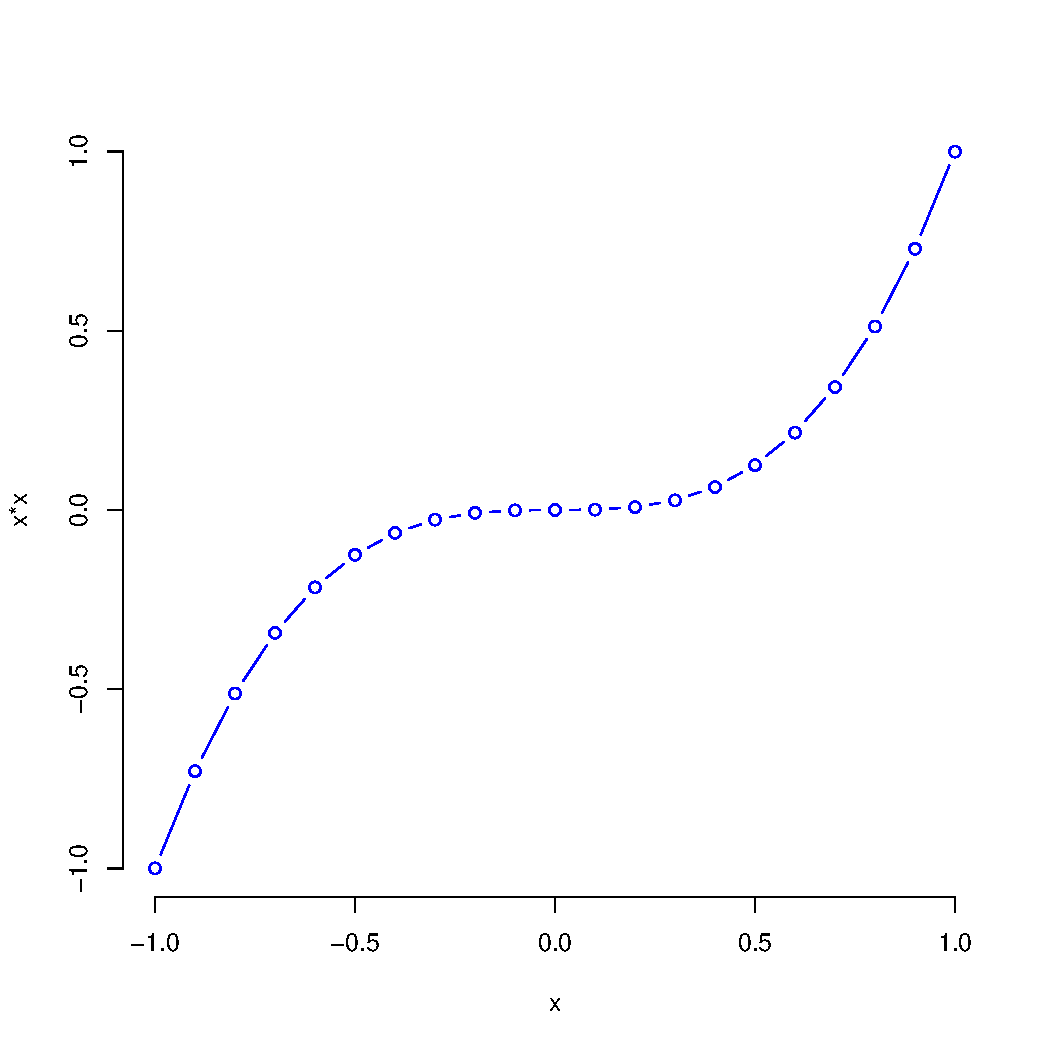
\includegraphics[width=.47\linewidth]{figure/unnamed-chunk-3-1} 

\end{knitrout}

\caption {Simple Plot of $f(x)=x^3$ Function}
\label{fig1}
\end {center}
\end {figure}




\subsection{Experiments}\label{experiments}

Now we can show how the function $f(x)=x^2$ looks like (Figure~\ref{fig2})

\begin{figure}[H] %start a figure
\begin{center}

\begin{knitrout}
\definecolor{shadecolor}{rgb}{0.969, 0.969, 0.969}\color{fgcolor}
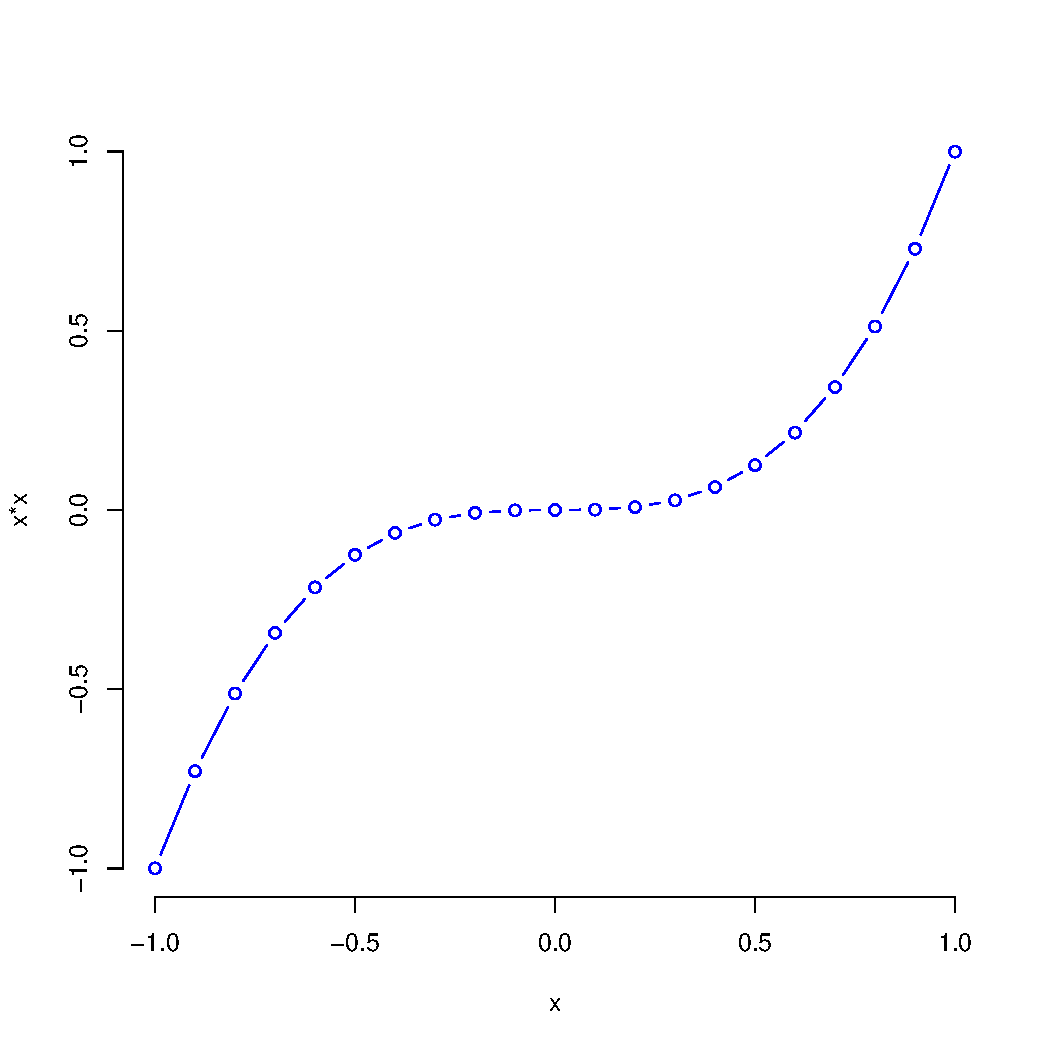
\includegraphics[width=.47\linewidth]{figure/unnamed-chunk-4-1} 

\end{knitrout}

\caption {Simple Plot of $f(x)=x^3$ Function}
\label{fig2}
\end {center}
\end {figure}


\section{Conclusion and Future Work}\label{cdsmote1}

%Edit here 
%\blindtext[2]





\section{Project Management}\label{mgt}

\subsection{Project Progress}
%Edit here 
%\blindtext[2]
% Pay attention to the code below including the chunk options 
% latex table generated in R 3.6.1 by xtable 1.8-4 package
% Tue Feb 25 18:15:58 2020
\begin{table}[ht]
\centering
\caption{Record of Team Meetings} 
\label{tab:one}
\begin{tabular}{llp{8cm}llll}
  \hline
No & Date & Topic & John & Ali & Ann & Mon \\ 
  \hline
1.00 & 2019-02-05 & Team Formation Formation Formation Formation Formation  & yes & yes & yes & yes \\ 
  2.00 & 2019-02-06 & Team Formation & yes & yes & yes & yes \\ 
  3.00 & 2019-02-07 & Team Formation & yes & yes & yes & yes \\ 
  4.00 & 2019-02-08 & Team Formation & yes & yes & yes & yes \\ 
  5.00 & 2019-02-09 & Team Formation & yes & yes & yes & yes \\ 
  6.00 & 2019-02-10 & Team Formation & yes & yes & yes & yes \\ 
  7.00 & 2019-02-11 & Team Formation & yes & yes & yes & yes \\ 
  8.00 & 2019-02-12 & Final Meeting & yes & yes & yes & yes \\ 
   \hline
\end{tabular}
\end{table}





\subsection{Peer-assessment}

%Edit here 
%\blindtext[2] \\

Same as we did with Table~\ref{tab:one}, we can also generate the peer-assessment table providing that we record things in an excel sheet. 

% latex table generated in R 3.6.1 by xtable 1.8-4 package
% Tue Feb 25 18:15:59 2020
\begin{table}[ht]
\centering
\caption{Peer Assessment out of 100} 
\label{tab:two}
\begin{tabular}{llllll}
  \hline
Peer.Review & Alex & Georgios & Karen & Roshi & Stuart \\ 
  \hline
Alex & 100 & 100 & 100 & 100 & 100 \\ 
  Georgios & 100 & 100 & 100 & 100 & 100 \\ 
  Karen & 100 & 100 & 100 & 100 & 100 \\ 
  Roshi & 100 & 100 & 100 & 100 & 100 \\ 
  Stuart & 100 & 100 & 100 & 100 & 100 \\ 
   \hline
\end{tabular}
\end{table}




\section*{References}\label{pubs}
\printbibliography[heading =none]

\end{document}
